\section{Systems of First-Order Linear Equations}\label{sec:firstorder}

\subsection{Classification of Differential Equations}

\begin{definition}
	Given some independent real variables $x_1, x_2, \ldots, x_n$ and some real-valued functions $y_1(x_j), y_2(x_j), \ldots, y_p(x_j)$, a system of differential equations is a system of equations relating them involving the derivatives $\p_j y_r, \p_i\p_j y_s, \ldots$ of the dependent variables:\footnote{In this case, the notation $x_j$ is used as a shorthand for the vector $\xt = (x_1, x_2, \ldots, x_n)$. In other cases where $j$ is specified, $x_j$ can be used to indicate the $j$th component of $\xt$.}
	\[
		\mathcal{F}_s[y_r, \p_j y_r, \ldots, x_j] = 0, \quad s = 1, \ldots, p.
	\]
\end{definition}

In other words, a differential equation is simply an equation relating a function and its derivatives.

\begin{eg}
	Some examples of differential equations are:
	\begin{equation*}
	\begin{split}
		y'(x) = 0 \\
		\ddot{y}(t) - \omega^2 y(t) = 0 \\
		\begin{cases} \dot{x}_1(t) = x_2(t) \\ \dot{x}_2(t) = -\sin(x_1(t)) \end{cases} \\
		(\p_x y)^2 + \tanh{x}\p_z y = e^{2x+z}.
	\end{split}
	\end{equation*}
\end{eg}

Differential equations may depend on \textbf{parameters}, like the real parameter $\omega$ in the second example. It is important to distinguish them from the independent variables (such as $t$ in the same example). This is usually clear from the context, but the defining feature of a parameter is that the differential equation does not involve any derivatives with respect to it. Nonetheless, solutions of differential equations depend on the parameters, and understanding this parametric dependence is an important part of analysing differential equations.

\subsubsection{ODEs vs. PDEs}

\begin{definition}
	Given the two sets $\{x_1, x_2, \ldots, x_n\}$ and $\{y_1(x_j), y_2(x_j), \ldots, y_p(x_j)\}$:
	\begin{enumerate}
		\item If $n=1$ (i.e. there is only one independent variable), we have an Ordinary Differential Equation (ODE) containing only ordinary derivatives, e.g. $\ddot{y}(t) - \omega^2 y(t) = 0$. 
		\item If $n>1$ (i.e. more than one independent variable), we have a Partial Differential Equation (PDE) containing partial derivatives, e.g. $(\p_x y)^2 + \tanh{x}\p_z y = e^{2x+z}$.
	\end{enumerate}
	If there is more than equation involving functions and there derivatives, we have a system of ODEs or PDEs. For example,
	\[
		\begin{cases} \dot{x}_1(t) = x_2(t) \\ \dot{x}_2(t) = -\sin(x_1(t)) \end{cases}
	\]
	is a system of two ODEs, since there are two equations and one independent variable, $t$.
\end{definition}

\subsubsection{Linear vs. Non-linear}
	
Consider ODEs with a single function of one variable $y(x)$. By collecting all the $y$-dependent terms, we can write the ODE as a condition on a (possibly $x$-dependent) map $L$ acting on $y$,
\[
	L[y] = f
\]
for some real function $f$. For example, $y''(x) - xy(x) = x^2$ corresponds to $L[y] = f$ with $L \equiv \frac{d^2}{dx^2} - x$ and $f(x) = x^2$.

\begin{definition}
	We say and ODE is \textbf{linear} if the associated map $L$ is linear, i.e. if it satisfies the property
	\[
		L[a_1 y_1 + a_2 y_2] = a_1 L[y_1] + a_2 L[y_2] \quad \forall a_1,a_2 \in \R
	\]
	and for any pair of functions $y_1$, $y_2$.
\end{definition}

In simple terms, linear ODEs and PDEs are those where the dependent variables $y_i(x_j)$ appear linearly, i.e. raised to the power of one. For example, $y''(x) + x^2 y'(x) = e^{2x}$ is a linear ODE, while $y'(x) + y(x)^2 = -\sin{x}$ is non-linear as it contains the $y(x)^2$ term.

Differential equations are also classified by \textbf{order}. The order of a differential equation is simply the highest-order derivative that it contains. For example, $y'' - xy = x^2$ is a second-order ODE.


\subsection{Introduction to Systems of First-Order ODEs}

In a system of first-order differential equations, we generally consider the independent variable $t$ and a set of dependent variables $x_i(t)$, established and connected as follows:
\begin{equation}\label{eq:fosystem}
	x_i'(t) = F_i(x_1, x_2, \ldots, x_n, t), \quad i = 1, 2, \ldots, n
\end{equation}

A system is said to be \vb{autonomous} if $\p_t F_i = 0$ for all $i$ (in other words, the equations are independent of $t$).

\begin{theorem}[Existence and Uniqueness]
	Let the functions $F_1, \ldots, F_n$ and partial derivatives $\p_{x_1}F_1, \ldots, \p_{x_n}F_1, \ldots, \p_{x_1}F_n, \ldots, \p_{x_n}F_n$ be continuous in the region $R$ defined by $\alpha \leq t \leq \beta$, $\alpha_i \leq x_i \leq \beta_i$, $\forall i$. Then for each point $(t_0, x_1^0, \ldots, x_n^0) \in R$, there exists an interval $[t_0-h, t_0+h]$ in which there is a unique solution $x_1 = \phi_1(t), \ldots, x_n = \phi_n(t)$ of \Cref{eq:fosystem} satisfying the initial condition $\phi_i(t_0) = x_i^0 \,\, \forall i$.
\end{theorem}

It is often useful to transform a higher-order differential equation into a system of first-order ODEs.

\begin{eg}
	Write the differential equation $y''' + 2(y')^2 + 3ty = 0$ as a system of first-order ODEs.
	
	We define new variables $x_1$, $x_2$ and $x_3$, with
	\begin{align*}
		x_1(t) &= y \\
		x_2(t) &= y' \\
		x_3(t) &= y''
	\end{align*}
	then it is clear that
	\begin{align*}
		x_1' &= y' = x_2 \\
		x_2' &= y'' = x_3
	\end{align*}
	and also that
	\[
	x_3' = y''' = -2(y')^2 - 3ty = -2x_2^2 - 3t x_1. 
	\]
	Thus the original ODE may be written as the following system:
	\begin{align*}
		x_1' &= x_2 \\
		x_2' &= x_3 \\
		x_3' &= -2x_2^2 - 3t x_1.
	\end{align*}
\end{eg}

The general method for transforming an arbitrary $n$th order ODE $y^{(n)}(t) = F(y, y', \ldots, y^{(n-1)}, t)$ into a system of first-order ODEs is as follows:
\begin{enumerate}
	\item Define $n$ new independent variables $x_1 = y$, $x_2 = y'$, ... $x_n = y^{(n-1)}$.
	\item Take derivatives:
	\begin{align*}
		x_1' &= x_2 \\
		x_2' &= x_3 \\
		&\vdots \\
		x_{n-1}' &= x_n \\
		x_n' &= y^{(n)} = F(y, \ldots, y^{(n-1)}, t).
		\intertext{\item Hence the system is}
		x_1' &= x_2 \\
		&\vdots \\
		x_n' &= F(x_1, \ldots, x_{n-1}, t).
	\end{align*}
\end{enumerate}

\begin{exercise}
	Consider the second-order ODE with parametric dependence on $m, \gamma \in \R$:
	\[
		mu'' + \gamma u' + ky = F(t).
	\]
	Convert this into a system of first-order ODEs.
\end{exercise}

\subsubsection{Geometric Interpretation}

Geometrically, we may visualise a system of first-order equations as a vector field. If the system is autonomous, then the vector field will be static over time, while if the system is not autonomous then the vector field will change over time.

The solutions to the system are tangential to the vectors - in order words, the solution trajectories follow the arrows (see \Cref{fig:geomsys}).

\begin{figure}[!ht]
	\centering
	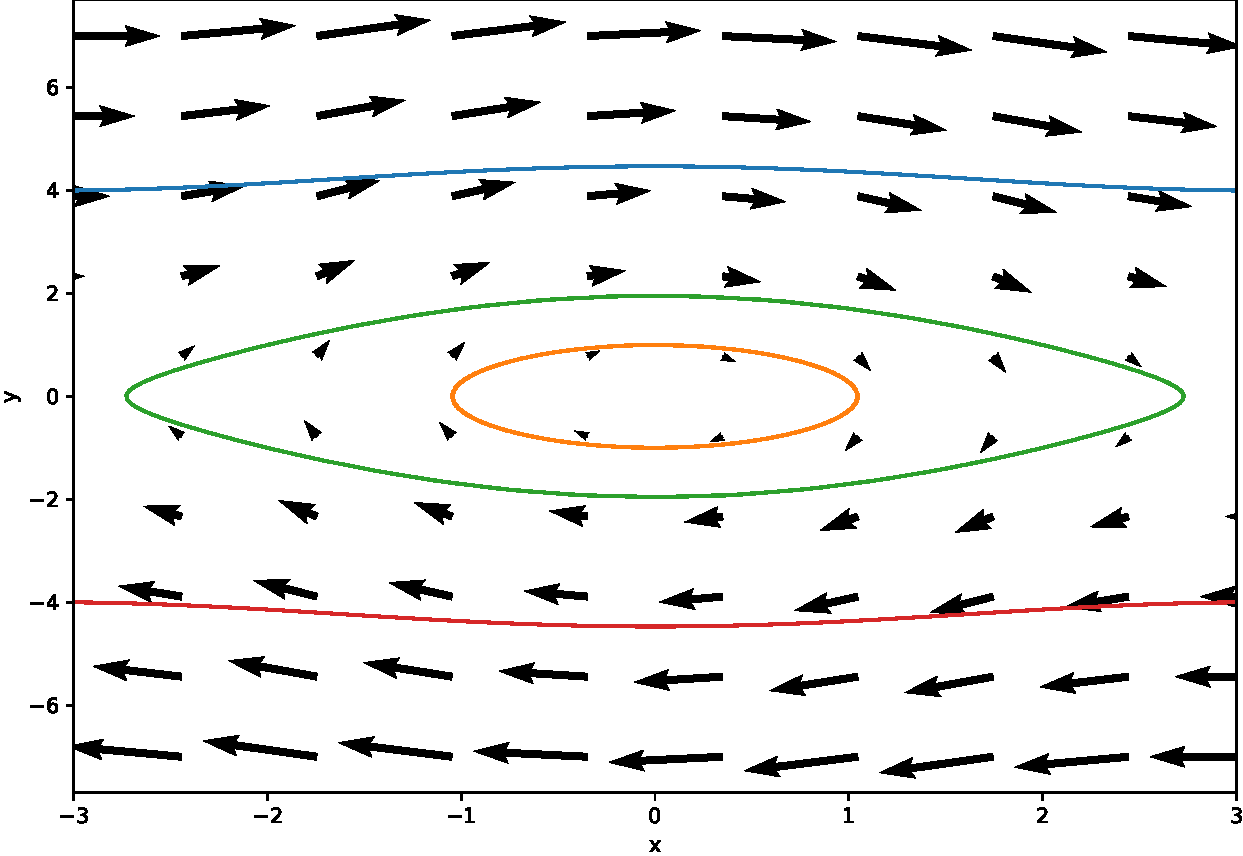
\includegraphics[width=0.7\textwidth]{vectorField.pdf}
	\caption{Direction field and selected solution trajectories for the system $x_0' = x_1$ and $x_1' = -\sin(x_0)$. Note that this is an example of an autonomous system.}
	\label{fig:geomsys}
\end{figure}


\subsection{Linear Systems of ODEs}

The general form of a linear system of ODEs is
\begin{equation}\label{eq:linearsystem}
	x_i'(t) = \sum_{j=1}^n P_{ij}(t) x_j(t) + g_i(t), \quad i = 1,\ldots,n.
\end{equation}

\begin{theorem}
	If $P_{ij}(t)$ and $g_i(t)$ are continuous in $[\alpha, \beta] \implies \exists t_0 \in (\alpha, \beta)$, there is a unique solution $x_t = \phi_i(t)$ in $[\alpha, \beta]$ solving \Cref{eq:linearsystem} and satisfying the initial condition $\phi_i(t_0) = x_i^0$.
\end{theorem}

For simplicity, we define the vector $\xt$ and matrix $P(t)$ as
\begin{equation}
	\xt = (x_1(t), x_2(t), \ldots, x_n(t)) \in \R^n \quad \text{and} \quad P(t) = \mat{P_{11}(t) & \cdots & P_{1n}(t) \\ \vdots & \ddots & \vdots \\ P_{n1}(t) & \cdots & P_{nn}(t)} \in \R^{n \times n}.
\end{equation}

Then \Cref{eq:linearsystem} may be written as
\begin{equation}\label{eq:linearsystemvector}
	\xtp = P(t) \xt + \gt.
\end{equation}

We say the system is homogeneous if $\vb{g} = \bm{0}$; otherwise, it is non-homogeneous or inhomogeneous. For now, we will only work with homogeneous systems, which we may write as $\vbx' = P\vbx$.

\begin{theorem}[Principle of Superposition]\label{thrm:superposition}
	If $\{\vbx^{(j)}(t)\}$, $j = 1, \ldots, p$ is a set of solutions,
	\begin{equation}\label{eq:gensol}
		\xt = \sum_{j=1}^p c_j \vbx^{(j)}(t), \quad c_j \in \R
	\end{equation}
	is also a solution.
\end{theorem}

\begin{proof}
	We have that $\vbx^{(j)}(t)$ is a solution of $\xtp = P(t) \xt$ (\Cref{eq:linearsystemvector}). Therefore
	\[
	\vbx^{(j)'}(t) = P(t) \vbx^{(j)}(t), \quad \forall j.
	\]
	Now, we find that
	\begin{align*}
		\xtp &= \sum_{j=1}^p c_j \vbx^{(j)'}(t)
		= \sum_{j=1}^p c_j P(t) \vbx^{(j)}(t) \\
		&= P(t) \sum_{j=1}^p c_j \vbx^{(j)}(t) \tag{Since $P(t)$ is indep. of $j$} \\
		&= P(t) \xt,
	\end{align*}
	i.e. $\xt$ satisfies the original ODE, making it a solution.
\end{proof}

\begin{remark}
	The Principle of Superposition only applies to homogeneous systems; that is, those of the form $\xtp = P\xt$.
\end{remark}

The space of solutions is a vector space of dimension $n$. To analyse the linear independence of $\{\vbx^{(j)}(t)\}, j = 1, \ldots, n$, we consider the following determinant
\begin{equation}\label{eq:wronskian}
	\det(\vbx^{(1)}(t), \vbx^{(2)}(t), \ldots, \vbx^{(n)}(t)) = \left| \begin{array}{cccc} x_1^{(1)} & x_1^{(2)} & \cdots & x_1^{(n)} \\ x_2^{(1)} & x_2^{(2)} & \cdots & x_2^{(n)} \\ \vdots & \vdots & \ddots & \vdots \\ x_n^{(1)} & x_n^{(2)} & \cdots & x_n^{(n)}
	\end{array} \right|
\end{equation}
Then, if this determinant is non-zero, the set of vectors are linearly independent. We call this determinant the \vb{Wronskian}, $W[\{\vbx^{(j)}(t)\}]$.

\begin{theorem}\label{thrm:fundamentalset}
	If $W[\{\vbx^{(j)}(t)\}] = W(t) \neq 0$ for $\alpha \leq t \leq \beta$, we say $\{\vbx^{(j)}(t)\}$ forms a fundamental set of solutions. Then, any solution may be written as a linear combination of the $\vbx^{(j)}$
	\[
	\xt = \sum_{j=1}^n c_j \vbx^{(j)}(t).
	\]
\end{theorem}

\begin{theorem}[Abel's Theorem]
	If $W(t_0) \neq 0$ for some $t_0$, then $W(t) \neq 0$ for all $\alpha \leq t \leq \beta$.
\end{theorem}

\begin{theorem}[Abel's Formula]
	The Wronskian satisfies
	\[
	W'(t) = \text{tr}(P(t)) W(t) = (P_{11} + \cdots + P_{nn}) W(t).
	\]
	Hence
	\[
	W(t) = e^{\int_{t_0}^t \text{tr} P(s) \,ds} W(t_0).
	\]
\end{theorem}

\begin{remark}
	Abel's Formula implies Abel's Theorem since if $W(t_0) \neq 0$, so too must $W(t) \neq 0$ since the exponential function is always non-zero.
\end{remark}

\begin{proof}
	We will use the definition of the derivative:
	\begin{equation}\label{eq:abelproof}
		W'(t) = \lim_{h\to 0} \frac{W(t+h) - W(t)}{h}.
	\end{equation}
	Note that the system of equations we are considering is homogeneous, i.e. $\xtp = P\xt$.
	
	Now we use the Taylor Expansion of $\vbx(t+h)$:
	\begin{align*}
		\vbx(t+h) &= \xt + h\xtp + O(h^2) \\
		&= \xt + hP(t)\xt + O(h^2) \tag{Using $\xtp = P\xt$} \\
		&= (I + hP(t))\xt + O(h^2)
	\end{align*}
	Then
	\begin{align*}
		W(t+h) &= \det\left(\vbx^{(1)}(t+h), \ldots, \vbx^{(n)}(t+h)\right) \\
		&= \det\left((I + hP(t))\vbx^{(1)}(t), \ldots, (I + hP(t))\vbx^{(n)}(t)\right) + O(h^2) \\
		&= \det\left[(I+hP(t))(\vbx^{(1)}(t), \ldots, \vbx^{(n)}(t))\right] + O(h^2) \\
		&= \det\left(I+hP(t)\right) \cdot \det\left(\vbx^{(1)}(t), \ldots, \vbx^{(n)}(t)\right) + O(h^2) \tag{Using $\det(AB) = \det(A)\det(B)$} \\
		&= \det\left(I+hP(t)\right) \cdot W(t) + O(h^2) \tag{By def. of Wronskian}
	\end{align*}
	
	Now looking at $\det\left(I+hP(t)\right)$:
	\begin{align*}
		\det\left(I+hP(t)\right) &= \left|\begin{array}{cccc}1+hP_{11} & hP_{12} & \cdots & hP_{1n} \\ hP_{21} & 1+hP_{22} & \cdots & hP_{2n} \\ \vdots & \vdots & \ddots & \vdots \\ hP_{n1} & hP_{n2} & \cdots & 1+hP_{nn} \\\end{array}\right| \\
		&= (1+hP_{11})\left|\begin{array}{cccc}hP_{12} & \cdots & hP_{1n} \\ \vdots & \ddots & \vdots \\hP_{n2} & \cdots & 1+hP_{nn} \\\end{array}\right| + O(h^2) \\
		&= (1+hP_{11})(1+hP_{22})\cdots (1+hP_{nn}) + O(h^2) \\
		&= 1 + hP_{11} + \cdots + hP_{nn} + O(h^2) \\
		&= 1 + h \text{tr}(P(t)) + O(h^2).
	\end{align*}
	Where all terms of the order $h^2$ or higher are collected under the umbrella of $O(h^2)$. Therefore
	\[
	W(t+h) = (1 + h \text{tr}(P(t))) W(t) + O(h^2)
	\]
	
	Finally, using this in \Cref{eq:abelproof}:
	\begin{align*}
		W'(t) &= \lim_{h\to 0} \frac{W(t+h) - W(t)}{h} \\
		&= \lim_{h\to 0} \frac{W(t) + h \text{tr}(P(t)) W(t) - W(t) + O(h^2)}{h} \\
		&= \lim_{h\to 0} \frac{h\text{tr}(P(t)) W(t)}{h} + \lim_{h\to 0}\frac{O(h^2)}{h} \\
		&= \text{tr}(P(t)) W(t).
	\end{align*}
	From which the formula for $W(t)$ follows easily.
\end{proof}

\subsection{Homogeneous Linear Systems with Constant Coefficients}\label{sec:homocc}

The aim of this section is to solve systems of $n$ first-order ODEs of the form $\xtp = A \xt$, $A \in \R^{n\times n}$, with $A$ a constant matrix.

To do this, we seek exponential solutions (similar to the method used for solving ODEs with constant coefficients in \Cref{sec:secondorderconst}); this is, those of the form
\begin{align*}
	\xt &= e^{rt} \xib \\
	\implies \xtp &= re^{rt} \xib = A e^{rt} \xib \\
	\implies (A-rI)\xib &= \bm{0}.
\end{align*}

In other words, we require that $r$ is an eigenvalue of $A$ and $\xib$ is the corresponding eigenvector. The $n$ eigenvalues then yield $n$ solutions to the system (if they all exist).\footnote{One might wonder how we come up with the idea for exponential solutions. We can derive this by starting with a simpler guess for the solutions of $\xt = f(t)\xib$ - simply a function of time multiplied by a constant vector $\xib$. Then we substitute this into the differential equation $\xtp = A \xt$ and obtain the equation
\[
	f'(t) \xib = f(t) A \xib \overset{f(t) \neq 0}{\implies} \frac{f'(t)}{f(t)}\xib = A\xib.
\]
Since there is no time-dependence on the right-hand side of this equation, $\frac{f'(t)}{f(t)}$ must be constant i.e. $\frac{f'(t)}{f(t)} = r$ and the equation above becomes $A\xib = r \xib$. We can then see that this is solved by $f(t) = e^{rt}$ and $\xib$ being an eigenvector of $A$ associated with the eigenvalue $r$. (Normally $f(t) = e^{rt}$ would contain an arbitrary constant $+C$, but since the eigenvector $\xib$ already contains an arbitrary constant of multiplication - $k\xib$ is also an eigenvector for $k \in \R \setminus \{0\}$ - 	there is no loss of generality by omitting the constant from $f(t)$.)}

Assuming the eigenvalues are all distinct, we have $n$ solutions, each of the form
\[
\vbx^{(j)}(t) = e^{r_j t} \xib_j, \quad j = 1, \ldots, n.
\]

We can see that these form a fundamental set, since
\begin{align*}
	W[\{\vbx^{(j)}(t)\}] &= \det(\vbx^{(1)}(t), \vbx^{(2)}(t), \ldots, \vbx^{(n)}(t)) \\
	&= \underbrace{e^{(r_1 + \cdots + r_n)t}}_{\neq 0} \det (\xib_1, \ldots, \xib_n)
\end{align*}
and $\det (\xib_1, \ldots, \xib_n) \neq 0$ since the eigenvectors associated with distinct eigenvalues are linearly independent. Therefore the Wronskian itself is non-zero, and we apply the result of \Cref{thrm:fundamentalset}.

Therefore the general solution may be written as
\begin{equation}\label{eq:generalsol}
	\xt = \sum_{j=1}^n c_j e^{r_jt} \xib_j.
\end{equation}

This holds provided that all eigenvalues are distinct ($r_i \neq r_j$ for $i \neq j$), \textbf{or} the algebraic multiplicity of each eigenvalue is equal to the geometric multiplicity.

\begin{eg}\label{eg:constsys1}
	Solve the system $\xtp = \mat{1 & 1 \\ 4 & 1} \xt$.
	
	We seek solutions of the form $\xt = e^{rt} \xib$, which as seen above requires that
	\begin{align*}
		(A-rI)\xib &= \bm{0} \\
		\implies \mat{1-r & 1 \\ 4 & 1-r} \xib &= \bm{0} \\
		\implies \det \mat{1-r & 1 \\ 4 & 1-r} &= 0 \\
		\implies (1-r)^2 -4 &= 0 \implies r = -1, 3.
	\end{align*}
	
	Now we find the eigenvectors associated with the eigenvalue $r_1=3$:
	\begin{align*}
		\mat{1-3 & 1 \\ 4 & 1-3} \xib = \mat{-2 & 1 \\ 4 & -2} \xib &= \bm{0} \\
		\implies \xib_1 &= \mat{1 \\ 2}.
	\end{align*}
	
	Similarly for $r_2=-1$:
	\begin{align*}
		\mat{1-(-1) & 1 \\ 4 & 1-(-1)} \xib = \mat{2 & 1 \\ 4 & 2} \xib &= \bm{0} \\
		\implies \xib_2 &= \mat{1 \\ -2}.
	\end{align*}
	
	Therefore the general solution may be written as
	\[
	\xt = c_1 e^{3t} \mat{1 \\ 2} + c_2 e^{-t} \mat{1 \\ -2}.
	\]
\end{eg}

\begin{remark}
	We can multiply through the vectors on the right-hand side of the general solution to write the equation as follows:
	\[
	\xt = \mat{x_1 \\ x_2} = \mat{c_1 e^{3t} + c_2 e^{-t} \\ 2c_1 e^{3t} - 2c_2 e^{-t}}.
	\]
\end{remark}

\begin{eg}
	Solve the system $\xtp = \mat{0 & 1 & 1 \\ 1 & 0 & 1 \\ 1 & 1 & 0} \xt$.
	
	As in \Cref{eg:constsys1}, we seek exponential solutions, and find the eigenvalues of the coefficient matrix to be $r_1 = -1$ and $r_2 = 2$. Note that the eigenvalue $r=-1$ has an algebraic multiplicity of 2.
	
	In finding eigenvectors, the eigenvector associated with $r=2$ is straightforward, with $\xib = \mat{1 \\ 1 \\ 1}$. For the eigenvalue $r=-1$, we find that the geometric multiplicity is 2, thus there are two linearly independent eigenvalues: $\xib = \mat{1 \\ 0 \\ -1}$ and $\xib = \mat{0 \\ 1 \\ -1}$.
	
	Putting this together, we may write the general solution as 
	\[
	\xt = c_1 e^{-t}\mat{1 \\ 0 \\ -1} + c_2 e^{-t} \mat{0 \\ 1 \\ -1} + c_3 e^{2t}\mat{1 \\ 1 \\ 1}.
	\]
\end{eg}

These two examples serve to illustrate the two different cases mentioned following \Cref{eq:generalsol} - where all eigenvalues are distinct or where algebraic and multiplicities are equal for all eigenvalues.

\begin{remark}
	With $\xt = \sum_{j=1}^n c_j e^{r_jt} \xib_j$, we may consider the behaviour of the solution as $t \to \infty$:
	\begin{itemize}
		\item $x \to 0$ if $\Re(r_j) < 0 \,\, \forall j$,
		\item $x \to \infty$ if $\Re(r_j) > 0 \,\, \forall j$,
		\item $x \to \infty$ for most initial conditions if $\exists j: \Re(r_j) > 0$.
	\end{itemize}
\end{remark}

\subsection{Homogeneous Linear Systems with Complex Eigenvalues}\label{sec:complexeigs}

In this section, we aim to solve the system $\xtp = A\xt$ with $A$ having complex conjugate eigenvalues. In addition, we will aim to write the solution in terms of real functions.\footnote{The methods of \Cref{sec:homocc} apply perfectly well to systems with complex eigenvalues; the only issue is that writing e.g. \[\xt = c_1 e^{-t/2 + it}\mat{1 \\ i} + c_2 e^{-t/2 - it}\mat{1 \\ -i}\] seems odd as a solution to a system given entirely in real numbers.}

First, observe that if $r_1 = \lambda + i\mu$ is an eigenvalue and $\xib_1$ is an eigenvector, so is $r_2 = r_i^* = \lambda - i\mu$, with $\xib_2 = \xib_1^*$.

So now we have two solutions: $\vbx_1(t) = e^{r_1t} \xib_1$ and $\vbx_2(t) = \vbx_1^*(t) = e^{r_1^*t} \xib_1^*$. Therefore in the $n=2$ case, the general solution of the whole system may be written as
\begin{equation*}\label{eq:complexgen}
	\xt = c_1 e^{r_1t} \xib_1 + c_2 e^{r_1^*t} \xib_1^*.
\end{equation*}

We wish to write the general solution in terms of real-valued functions instead of $\vbx_1(t)$ and $\vbx_1^*(t)$. We can do this by taking the two solutions to be the real and imaginary parts of $\vbx_1(t)$, since
\begin{equation*}
	\begin{alignedat}{2}
		\widetilde{\vbx}_1 &= \Re(\vbx_1(t)), \hspace{50pt} \widetilde{\vbx}_2 &&= \Im(\vbx_1(t)) \\
		&= \frac{x_1 + x_1^*}{2} &&= \frac{x_1 - x_1^*}{2i} \\
		&= \frac{x_1 + x_2}{2} &&= \frac{x_1 - x_2}{2i}
	\end{alignedat}
\end{equation*}
In other words, the real and imaginary parts of $\vbx_1(t)$ may be written as a linear combination of the two original solutions $\vbx_1(t)$ and $\vbx_2(t)$, thus are also a solution by the Principle of Superposition (\Cref{thrm:superposition}).

\begin{eg}
	Solve the system $\xtp = \mat{-\sfrac12 & 1 \\ -1 & -\sfrac12} \xt$, expressing your answer in terms of real functions.
	
	As before, we see exponential solutions of the form $\xt = e^{rt} \xib$, which requires that
	\begin{align*}
		\det \mat{-\frac12 -r & 1 \\ -1 & -\frac12 -r} &= 0 \\
		\implies \left(\frac12 + r\right)^2 + 1 &= 0 \\
		\implies r &= -\frac12 \pm i.
	\end{align*}
	
	We now find the eigenvector associated with the eigenvalue $r = -\frac12 + i$:
	\[
	\mat{-i & 1 \\ -1 & -i}\xib = 0 \implies \xib_1 = \mat{1 \\ i}.
	\]
	The eigenvector $\xib_2$ is the conjugate of $\xib_1$, so the general solution to the system is
	\[
	\xt = c_1 e^{-t/2 + it}\mat{1 \\ i} + c_2 e^{-t/2 - it}\mat{1 \\ -i}.
	\]
	
	However, we would rather use $\widetilde{\vbx}_1 = \Re(\vbx_1(t))$ and $\widetilde{\vbx}_2 = \Im(\vbx_1(t))$, so we write
	\begin{align*}
		\vbx_1(t) = e^{-t/2 + it}\mat{1 \\ i} &= e^{-t/2}(\cos t + i\sin t)\mat{1 \\ i} \\
		&= e^{-t/2}\mat{\cos t + i\sin t \\ i\cos t -\sin t}
	\end{align*}
	Taking the real and imaginary parts of this solution yields
	\[
	\widetilde{\vbx}_1 = e^{-t/2}\mat{\cos t \\ -\sin t} \quad\text{and}\quad \widetilde{\vbx}_2 = e^{-t/2}\mat{\sin t \\ \cos t}
	\]
	and a general solution of
	\[
	\xt = d_1 e^{-t/2}\mat{\cos t \\ -\sin t} + d_2 e^{-t/2}\mat{\sin t \\ \cos t}.
	\]
\end{eg}


\subsection{Matrix Methods}

\subsubsection{Fundamental Matrices}

\begin{definition}
	A fundamental matrix $\Psi(t)$ is an $n \times n$ matrix with fundamental solutions $\vbx^{(i)}$ as columns:
	\[
		\Psi(t) = (\vbx^{(1)}(t), \ldots, \vbx^{(n)}(t)) = \mat{x_1^{(1)} & x_1^{(2)} & \cdots & x_1^{(n)} \\ x_2^{(1)} & x_2^{(2)} & \cdots & x_2^{(n)} \\ \vdots & \vdots & \ddots & \vdots \\ x_n^{(1)} & x_n^{(2)} & \cdots & x_n^{(n)}}.
	\]
\end{definition}

Properties of the fundamental matrix:
\begin{itemize}
	\item $\det \Psi(t) = W(t) \neq 0$ because $\vbx^{(i)}$ form a fundamental set (see also \Cref{eq:wronskian}).
	\item{Considering the general solution in \Cref{eq:gensol},
		\begin{align*}
			\xt = \sum_{j=1}^p c_j \vbx^{(j)}(t) = (\vbx^{(1)}(t), \ldots, \vbx^{(n)}(t)) \mat{c_1 \\ \vdots \\ c_n} = \Psi(t) \bm{c}
		\end{align*}
		i.e. the general solution is given by the fundamental matrix multiplied by a vector of constants. Indeed, by \Cref{thrm:fundamentalset}, we have that \emph{any} solution may be written this way.}
	\item $\Psi'(t) = A \Psi(t)$ i.e. $\Psi(t)$ is a solution of the system of ODEs.
	\item $\xt = \Psi(t) \Psi^{-1}(t_0) \vbx_0$ solves $\xtp = A\xt$, with $\vbx(t_0) = \vbx_0$.
\end{itemize}

\begin{eg}\label{eg:fundamentalmatrix}
	Consider the system $\xtp = \mat{1 & 2 \\ 0 & 3} \xt$.
	
	We can easily solve the system (this is left as an exercise) to find the general solution to be
	\[
	\xt = c_1 e^t \mat{1 \\ 0} + c_2 e^{3t} \mat{1 \\ 1}
	\]
	Therefore the fundamental matrix is
	\[
	\Psi(t) = \mat{e^t & e^{3t} \\ 0 & e^{3t}}.
	\]
	Note that we can also check that $\Psi'(t) = A\Psi(t)$ (exercise!)
\end{eg}

It is important to note that the fundamental matrix of a system is \textbf{not} unique. Indeed, any matrix with its columns being linearly independent solutions to the system of ODEs is a valid fundamental matrix, e.g. $\mat{e^t & -3e^{3t} \\ 0 & -3e^{3t}}$ and $\mat{e^t & e^{3t}-2e^t \\ 0 & e^{3t}}$ for the system in the above example. This may be summarised in the statement that $\Psi(t) \cdot B$ is a fundamental matrix for constant matrix $B$.

\subsubsection{Matrix Exponentiation}

Recall that, for some scalar $a \in \R$, $e^a$ may be defined by power series:
\[
e^a = \sum_{k=0}^{\infty} \frac{a^k}{k!}.
\]

For a matrix $A$, we define $e^{At}$ analogously:
\[
e^{At} = \sum_{k=0}^{\infty} \frac{(At)^k}{k!} = I + At + \frac{A^2t^2}{2!} + \frac{A^3t^3}{3!} + \cdots
\]

Alternatively,
\[
	e^{At} = \lim_{n\to\infty} \left(I + \frac{1}{n}A\right)^n.
\]

Properties of $e^{At}$:
\begin{itemize}
	\item $e^{At} = I$ at $t=0$.
	\item $\frac{d}{dt}(e^{At}) = A e^{At}$, i.e. $e^{At} = \Psi(t)$ for $\Psi(0) = I$.\footnote{Checking this using the series definition of $e^{At}$ is a good exercise.}
	\item The solution of $\xtp = A\xt$ such that $\vbx(0) = \vbx_0$ is $\xt = e^{At} \vbx(0)$. This is because $\xt = \Psi(t) \Psi^{-1}(0) \vbx_0$ and $\Psi^{-1}(0) = I$ for $\Psi(t) = e^{At}$ since $e^{At} = I$ at $t=0$.
\end{itemize}

\begin{eg}
	Returning to the example in \Cref{eg:fundamentalmatrix}, we found that a fundamental matrix for the system $\xtp = \mat{1 & 2 \\ 0 & 3} \xt$ was $\Psi(t) = \mat{e^t & e^{3t} \\ 0 & e^{3t}}$.
	
	In order to have $e^{A\cdot 0} = I$, we require that
	\[
	e^{At} = \Psi(t) \Psi^{-1}(0).
	\]
	Determining $\Psi^{-1}(0)$:
	\[
	\Psi(0) = \mat{1 & 1 \\ 0 & 1} \implies \Psi^{-1}(0) = \mat{1 & -1 \\ 0 & 1}.
	\]
	Therefore
	\[
	e^{At} = \Psi(t) \Psi^{-1}(0) = \mat{e^t & e^{3t} \\ 0 & e^{3t}} \mat{1 & -1 \\ 0 & 1} = \mat{e^t & e^{3t}-e^t \\ 0 & e^{3t}}.
	\]
\end{eg}

\textbf{Summary:} A fundamental matrix is a matrix with its columns being linearly independent solutions to the system $\xtp = A\xt$. The matrix $e^{At}$ is a fundamental matrix, with the additional condition that $e^{At}$ is equal to the identity matrix when $t=0$.\footnote{3Blue1Brown has an excellent video relating to matrix exponentials and systems of differential equations that I would highly recommend: click \href{https://www.youtube.com/watch?v=O85OWBJ2ayo}{here}.}

\subsubsection{Matrix Exponentiation and Diagonalisation}\label{sec:diag}

Recall that the $n \times n$ matrix $A$ is diagonalisable if it has $n$ independent eigenvectors $\xib^{(i)}$, with $A \xib^{(i)} = r_i \xib^{(i)}$.

We construct a matrix with the eigenvectors as columns
\[
	T = \left(\xib ^{(1)}, \ldots, \xib ^{(n)}\right) = \mat{\xib_1^{(1)} & \xib_1^{(2)} & \cdots & \xib_1^{(n)} \\ \xib_2^{(1)} & \xib_2^{(2)} & \cdots & \xib_2^{(n)} \\ \vdots & \vdots & \ddots & \vdots \\ \xib_n^{(1)} & \xib_n^{(2)} & \cdots & \xib_n^{(n)}}.
\]
The Matrix $AT$ has columns equal to $A \xib^{(i)} = r_i \xib^{(i)}$, thus
\begin{align*}
	AT &= \mat{r_1\xib_1^{(1)} & \xib_1^{(2)} & \cdots & r_n\xib_1^{(n)} \\ r_1\xib_2^{(1)} & \xib_2^{(2)} & \cdots & r_n\xib_2^{(n)} \\ \vdots & \vdots & \ddots & \vdots \\ r_1\xib_n^{(1)} & \xib_n^{(2)} & \cdots & r_n\xib_n^{(n)}} = T \mat{r_1 & 0 & \cdots & 0 \\ 0 & r_2 & \cdots & 0 \\ \vdots & \vdots & \ddots & \vdots \\ 0 & 0 & \cdots & r_n} \\
	&= T \text{diag}(r_1, \ldots, r_n) \equiv TD \\
	&\implies D = T^{-1}AT.
\end{align*}

The relation $D = T^{-1}AT$ corresponds to a change of basis $\vbx = t\vb{y}$, which can be seen from the fact that
\[
	\vbx t\vb{y} \implies T \frac{d\vb{y}}{dt} = AT\vb{y} \implies \frac{d\vb{y}}{dt} = T^{-1}AT \vb{y} = D\vb{y}.
\]
The fundamental matrix of the system under the change of variables is
\[
	Q(t) = e^{Dt} = \text{diag}(e^{r_1t}, e^{r_2t}, \ldots, e^{r_nt}) = \mat{e^{r_1t} & 0 & \cdots & 0 \\ 0 & e^{r_2t} & \cdots & 0 \\ \vdots & \vdots & \ddots & \vdots \\ 0 & 0 & \cdots & e^{r_nt}}.
\]
Then the fundamental matrix in the original variables $\vbx$ is
\[
	\Psi(t) = TQ(t) = T \text{diag}(e^{r_1t}, e^{r_2t}, \ldots, e^{r_nt}),
\]
and the exponential matrix is
\[
	e^{At} = \Psi(t) \Psi^{-1}(0) = TQT^{-1} = T \text{diag}(e^{r_1t}, e^{r_2t}, \ldots, e^{r_nt}) T^{-1}.
\]

\begin{eg}
	Compute $e^{At}$ for $A = \mat{1 & 1 \\ 4 & 1}$.
	
	We can easily find the eigenvalues to be $r=-1,3$ and the corresponding eigenvectors to be $\mat{1 \\ -2}$ and $\mat{1 \\ 2}$.
	
	So
	\[
	T = \mat{1 & 1 \\ -2 & 2} \quad \text{and} \quad T^{-1} = \mat{\sfrac{1}{2} & \text{-}\sfrac{1}{4} \\ \sfrac{1}{2} & \sfrac{1}{4}}
	\]
	then
	\[
	e^{At} = Te^{Dt}T^{-1} = \mat{1 & 1 \\ -2 & 2} \mat{e^{-t} & 0 \\ 0 & e^{3t}} \mat{\sfrac{1}{2} & \text{-}\sfrac{1}{4} \\ \sfrac{1}{2} & \sfrac{1}{4}} = \mat{\frac12(e^{-t}+e^{3t}) & \frac14(e^{3t}-e^{-t}) \\ e^{3t}-e^{-t} & \frac12(e^{-t}+e^{3t})}
	\]
\end{eg}


\subsection{Homogeneous Linear Systems with Repeated Eigenvalues}\label{sec:repeatedeigs}

We will now solve systems $\xtp = A\xt$ where the matrix $A$ has repeated eigenvalues with geometric multiplicity less than algebraic multiplicity. This is best illustrated with an example:

\begin{eg}\label{eg:repeigs}
	Solve the system $\xtp = A\xt$ with $A = \mat{1 & -1 \\ 1 & 3}$.
	
	As usual, we try exponential solutions of the form $\xt = e^{rt}\xib$, and find the only eigenvalue of the matrix to be $r=2$ with algebraic multiplicity 2. Now to find the associated eigenvector(s):
	\[
	\mat{-1 & -1 \\ 1 & 1}\xib = 0 \implies \xib = \mat{1 \\ -1}.
	\]
	Therefore one solution is $\vbx^{(1)}(t) = e^{2t}\mat{1 \\ -1}$, but what is the other solution?
	
	For the second solution, we try
	\[
	\xt = te^{2t}\xib + e^{2t}\etab.
	\]
	Substituting this into the equation for the system, we get
	\[
	\xtp = e^{2t}\left[(2t+1)\xib + 2\etab\right] = A(te^{2t}\xib + e^{2t}\etab).
	\]
	Cancelling the $e^{2t}$ and comparing the coefficients of $t$:
	\[
	2\xib = A\xib \implies (A-2I) \xib = \bm{0}
	\]
	Which is precisely the eigenvalue problem we already solved. Now comparing the coefficients of $t^0$:
	\begin{align*}
		\xib + 2\etab = A\etab \implies (A-2I)\etab &= \xib \\ \mat{-1 & -1 \\ 1 & 1}\etab &= \mat{1 \\ -1} \\
		\etab &= \mat{-1 \\ 0} + k\mat{1 \\ -1}
	\end{align*}
	$\etab$ is known as a \vb{generalised eigenvector}.\footnote{It is called a generalised eigenvector since $(A-rI)\etab = \xib \implies (A-rI)^2\etab = \bm{0}$; a generalised eigenvector is defined as the vector $\vbx$ for which $(A-\lambda I)^p = \bm{0}$ for some positive integer $p$.} Observe that we may add any scalar multiple of the eigenvector $\xib$ to $\etab$ since $(A-2I)\xib = \bm{0}$ thus this addition will not affect the RHS of the equation $(A-2I)\etab = \xib$.
	
	We can now write the second solution as
	\[
	\vbx^{(2)}(t) = e^{2t}\left(t\mat{1 \\ -1} + \mat{-1 \\ 0} + k\mat{1 \\ -1}\right).
	\]
	Therefore the general solution is
	\[
	\xt = c_1 e^{2t}\mat{1 \\ -1} + c_2 e^{2t}\left(t\mat{1 \\ -1} + \mat{-1 \\ 0} + k\mat{1 \\ -1}\right).
	\]
	Note that without loss of generality, we can set $k=0$ since $c_2 k e^{2t}\mat{1 \\ -1}$ is just a multiple of the first term in the general solution. therefore a better general solution is
	\[
	\xt = c_1 e^{2t}\mat{1 \\ -1} + c_2 e^{2t}\left(t\mat{1 \\ -1} + \mat{-1 \\ 0}\right).
	\]
\end{eg}

\begin{exercise}
	Check that $\vbx^{(1)}(t)$ and $\vbx^{(2)}(t)$ form a fundamental set of solutions by calculating the Wronskian.
\end{exercise}

In general, the process for solving systems with repeated eigenvalues and too few eigenvectors is to construct the following independent solutions:
\begin{equation*}
	\begin{alignedat}{2}
		\vbx^{(1)}(t) &= \xib e^{rt} \qquad &&(A-rI)\xib = \bm{0} \\
		\vbx^{(2)}(t) &= (\xib t + \etab)e^{rt} \qquad && (A-rI)\etab = \xib \\
		\vbx^{(3)}(t) &= (\xib \frac{t^2}{2} + \etab t + \bm{\zeta})e^{rt} \qquad &&(A-rI)\bm{\zeta} = \etab \cdots
	\end{alignedat}
\end{equation*}

\subsubsection{Connection to Matrix Methods and Jordan Form}

Returning to the system in \Cref{eg:repeigs} and its general solution, we can find the fundamental matrix to be
\[
\Psi(t) = \mat{e^{2t} & (t-1)e^{2t} \\ -e^{2t} & -te^{2t}}.
\]
Then
\[
\Psi(0) = \mat{1 & -1 \\ -1 & 0}	\implies \Psi^{-1}(0) = \mat{0 & -1 \\ -1 & -1},
\]
so
\[
e^{At} = \Psi(t)\Psi^{-1}(0) = \mat{(1-t)e^{2t} & -te^{2t} \\ te^{2t} & (t+1)e^{2t}}.
\]

The Jordan form is an upper triangular matrix with the eigenvalues on its main diagonal, a diagonal consisting entirely of ones above the main diagonal (superdiagonal), and zero entries everywhere else:
\[
J_r = \mat{r & 1 \\ 0 & r}, \mat{r & 1 & 0 \\ 0 & r & 1 \\ 0 & 0 & r}, \cdots
\]

We illustrate some cases in which the Jordan form appears using $2 \times 2$ matrices, still using the system in \Cref{eg:repeigs}.

First, let
\[
T = (\xib, \etab) = \mat{1 & -1 \\ -1 & 0}.
\]
Then we find that
\[
T^{-1}AT = \mat{0 & -1 \\ -1 & -1} \mat{1 & -1 \\ 1 & 3} \mat{1 & -1 \\ -1 & 0} = \mat{2 & 1 \\ 0 & 2} = J_2.
\]

Now we shall compute $e^{J_rt}$. This is useful since $T^{-1}AT = J_r \implies e^{At} = Te^{J_rt}T^{-1}$. Note that $e^{A+B} = e^A e^B$ provided that $AB = BA$. We have
\[
J_r = \mat{r & 1 \\ 0 & r} = \mat{r & 0 \\ 0 & r} + \mat{0 & 1 \\ 0 & 0}
\]
Then
\[
e^{\mat{r & 0 \\ 0 & r}t} = \mat{e^{rt} & 0 \\ 0 & e^{rt}}
\]
and using the series definition of $e^{At}$,
\[
e^{\mat{0 & 1 \\ 0 & 0}t} = I + \mat{0 & t \\ 0 & 0} + \cancelto{0}{\frac12\mat{0 & t \\ 0 & 0}^2 + \cdots} = \mat{1 & t \\ 0 & 1}
\]
where higher powers are discarded since the matrix $\mat{0 & t \\ 0 & 0}$ is nilpotent.

So
\[
e^{J_rt} = \mat{e^{rt} & 0 \\ 0 & e^{rt}} \mat{1 & t \\ 0 & 1} = \mat{e^{rt} & te^{rt} \\ 0 & e^{rt}} = e^{rt} \mat{1 & t \\ 0 & 1}.
\]

In addition, a similar procedure may be used to find that, for a $3 \times 3$ Jordan form matrix $J_r$,\footnote{In fact, for the general $n \times n$ case, \[e^{J_rt} = e^{rt}\mat{1 & t & t^2/2 & \dots & t^{n-1}/(n-1)! \\ 0 & 1 & t & \dots & t^{n-2}/(n-2)! \\ \vdots & \vdots & \vdots & \ddots & \vdots \\ 0 & 0 & 0 & \dots & 1}.\] The proof of this is of course left as an exercise.}
\[
e^{J_rt} = e^{rt} \mat{1 & t & \frac{t^2}{2} \\ 0 & 1 & t \\ 0 & 0 & 1}.
\]


\subsubsection{Two More Examples}

\begin{eg}
	Solve the system $\xtp = \mat{3 & 1 \\ -4 & -1}\xt$.
	
	Through the usual process, we find the eigenvalue to be $r=1$ with algebraic multiplicity 2, and the corresponding eigenvector to be $\xib = \mat{1 \\ -2}$ i.e. with geometric multiplicity 1.
	
	Therefore we try a second solution $\vbx^{(2)}(t) = e^t(t\xib + \etab)$. This leads to the generalised eigenvector problem
	\begin{align*}
		(A-I)\etab &= \xib \\
		\mat{2 & 1 \\ -4 & -2}\etab &= \mat{1 \\ -2} \\
		\etab &= \mat{\sfrac{1}{2} \\ 0} + k\mat{1 \\ -2}
	\end{align*}
	Taking $k=0$ in the second solution, we find the following general solution:
	\[
	\xt = c_1 e^t \mat{1 \\ -2} + c_2 e^t \left(t\mat{1 \\ -2} + \mat{\sfrac{1}{2} \\ 0}\right).
	\]
\end{eg}

\begin{eg}
	Solve the system $\xtp = \mat{5 & -3 & -2 \\ 8 & -5 & -4 \\ -4 & 3 & 3}\xt$.
	
	Through the usual methods, we find the only eigenvalue to be $r=1$ with algebraic multiplicity 3. Now looking for the eigenvectors:
	\[
	\mat{4 & -3 & -2 \\ 8 & -6 & -4 \\ -4 & 3 & 2}\xib = \bm{0}.
	\]
	The rows of this matrix are all multiples of one another, so in looking for eigenvalues $\xib = \mat{x \\ y \\z}$, the only constraint is that $4x-3y-2z = 0$. Setting $x=0$ and $y=0$ respectively, we can find two linearly independent eigenvectors to be $\xib^{(1)} = \mat{1 \\ 0 \\ 2}$ and $\xib^{(2)} = \mat{0 \\ 2 \\ -3}$.
	
	Therefore two independent solutions are
	\[
	\vbx^{(1)}(t) = e^t\mat{1 \\ 0 \\ 2} \quad \text{and} \quad \vbx^{(2)}(t) = e^t\mat{0 \\ 2 \\ -3}.
	\]
	
	We will now try and find a third solution of the form
	\[
	\vbx^{(3)}(t) = e^t\left(t\left(a\xib^{(1)} + b\xib^{(2)}\right) + \etab \right).
	\]
	Substituting this into the equation for the system:
	\[
	\vbx^{(3)}(t) = e^t\left[t\left(a\xib^{(1)} + b\xib^{(2)}\right) + \etab + a\xib^{(1)} + b\xib^{(2)}\right] = Ae^t\left(t\left(a\xib^{(1)} + b\xib^{(2)}\right) + \etab\right).
	\]
	Cancelling the $e^t$ and equating the terms in $t$:
	\[
	Ae^t\left(a\xib^{(1)} + b\xib^{(2)}\right) = a\xib^{(1)} + b\xib^{(2)},
	\]
	which is satisfied since $\xib^{(1)}$ and $\xib^{(2)}$ are eigenvectors with corresponding eigenvalue $r=1$.
	
	Now comparing the terms in $t^0$:
	\begin{align*}
		A\etab &= \etab + a\xib^{(1)} + b\xib^{(2)} \\
		\implies (A-I)\etab &= a\xib^{(1)} + b\xib^{(2)} \\
		\implies \mat{4 & -3 & -2 \\ 8 & -6 & -4 \\ -4 & 3 & 2}\etab &= a\mat{1 \\ 0 \\ 2} + b\mat{0 \\ 2 \\ -3} = \mat{a \\ 2b \\ 2a-3b}
	\end{align*}
	We can find a compatibility condition between the elements of the vector $\mat{a \\ 2b \\ 2a-3b}$ based on the relation between the rows of the matrix $\mat{4 & -3 & -2 \\ 8 & -6 & -4 \\ -4 & 3 & 2}$ I.e, the second row is twice the first row, so $2a = 2b \iff a=b$, and the third row is the negative of the first, so $3b-2a = a$. Taking for simplicity $a=b=1$,
	\begin{align*}
		\mat{4 & -3 & -2 \\ 8 & -6 & -4 \\ -4 & 3 & 2}\etab = \mat{1 \\ 2 \\ -1}
	\end{align*}
	With $\etab = \mat{x \\ y \\ z}$ this gives a condition that $4x-3y-2z = 1$, so setting $y=z=0$ and recalling that the generalised eigenvector may contain any scalar multiple of the original eigenvectors, we find that
	\[
	\etab = \mat{\sfrac{1}{4} \\ 0 \\ 0} + k\mat{1 \\ 0 \\ 2} + l\mat{0 \\ 2 \\ -3}, \quad k,l \in \R.
	\]
	Taking $k=l=0$, the simplest form of the general solution is
	\[
	\xt = c_1 e^t \mat{1 \\ 0 \\ 2} + c_2 e^t \mat{0 \\ 2 \\ -3} + c_3 e^t \mat{t + \sfrac{1}{4} \\ 2t \\ -t}.
	\]
\end{eg}


\subsection{Non-homogeneous Linear Systems}

In this section, we turn to the Non-homogeneous system:
\[
\xtp = P(t) \xt + \gt
\]
where $P(t)$ is an $n \times n$ matrix and $\gt$ is the $n \times 1$ vector that makes the system non-homogeneous. The general solution of this system can be given by:
\begin{equation}
	\xt = \vbx_h(t) + \vbx_p(t)
\end{equation}

where $\vbx_h(t)$ is the general solution of the homogeneous system and $\vbx_p(t)$ is the particular solution of the non-homogeneous system. Note that this is essentially the same as when solving a single non-homogeneous ODE such as $y'' + 2y' + 5y = 2 e^t$.

Now, we aim to find the particular solution $\vbx_p(t)$ to the non-homogeneous system. We will mainly focus on systems $\xtp = A\xt + \gt$, i.e. those which have constant coefficients instead of a matrix $P(t)$ which is dependent on $t$. There are three methods to solve this:
\begin{itemize}
	\item Diagonalisation, for constant coefficients $P(t) = A$, any $\gt$.
	\item Method of undetermined coefficients, for constant coefficients $P(t) = A$, and where $\gt$ contains only exponential, polynomial, sine or cosine terms, or sums or products of these.
	\item Variation of parameters for any $P(t)$, any $\gt$.
\end{itemize}


\subsubsection{Diagonalisation}

Consider systems of the form
\begin{equation}
	\xtp = A \xt + \gt
\end{equation} 
where A is an $n \times n$ diagonalisable constant matrix. Let
\[
T = \left(\xib ^{(1)}, \ldots, \xib ^{(n)}\right) \quad \text{and} \quad \vbx = T \bm{y}.
\]
Then we have,
\begin{align*}
	\vbx' = T \bm{y}' &= A \vbx + \gt \\
	\implies T \bm{y}' &= A T \bm{y} + \gt
\end{align*}
We multiply by $T^{-1}$ to get:
\begin{equation}\label{eq:diagdecoupled}
	\bm{y}' = T^{-1} A T \bm{y} + T^{-1} \gt
\end{equation}
By \Cref{sec:diag}, recall $T^{-1} A T = \text{diag}(r_1,\ldots,r_n) = D$. Then we obtain a system of uncoupled ODEs:
\[
{y_i}' = r_i y_i + h_i(t)
\]
where $\bm{h}(t) = T^{-1} \gt$. Rearranging the terms and multiplying by $e^{-r_i t}$ (i.e. solving the ODE by integrating factors):
\begin{equation}\label{eq:diagsol}
	\begin{alignedat}{1}
		e^{-r_i t}(y_i' - r_i y_i) &= h_i e^{-r_i t} \\
		\implies (e^{-r_i t} y_i)' &= h_i e^{-r_i t} \\
		\implies e^{-r_i t} y_i &= c_i + \int^t_{t_0} h_i(s) e^{-r_i s} \,ds \\
		\implies y_i(t) &= c_i e^{r_i t} + e^{r_i t} \int^t_{t_0} h_i e^{-r_i s} \,ds
	\end{alignedat} 
\end{equation}

The solution $\xt$ is obtained by multiplying the matrix $T$ with $\bm{y}(t)$, where each component of $\bm{y}$ is given by the last line of \Cref{eq:diagsol}. The first term $c_i e^{r_i t}$ gives the general solution of the homogeneous equation $\xtp = A\xt$, while the second term yields the particular solution of the non-homogeneous system.

\begin{eg}\label{eg:nonhom}
	Solve the system $\xtp = A \xt + \gt = \mat{-2 & 1 \\ 1 & -2} \xt + \mat{2 e^{-t} \\ 3t}$
	
	The homogeneous solution is given by: $\vbx_h(t) = e^{rt} \xib$. By solving to find the eigenvalues, we find that $r$ satisfies the equation:
	\[
	(r+2)^2 -1=0 \implies r_1 = -1, r_2 = -3
	\] 
	The eigenvector corresponding to $r_1 = -1$ is $\xib^{(1)} = \mat{1 \\ 1}$ and the eigenvector corresponding to $r_2 = -3$ is $\xib^{(2)} = \mat{1 \\ -1}$. 
	
	Hence,
	\[
	\vbx_h(t) = c_1 e^{-t} \mat{1 \\ 1} + c_2 e^{-3t} \mat{1 \\ -1}
	\]
	Now we calculate the particular solution. Consider the matrix
	\[
	T = \left(\xib^{(1)}, \ldots, \xib^{(n)}\right) = \mat{1 &1 \\ 1 &-1}
	\]
	and let $\vbx = T \bm{y}$.
	
	Note that 
	\[
	T^{-1} = -\frac{1}{2} \mat{-1 & -1 \\ -1 & 1} = \mat{\sfrac{1}{2} & \sfrac{1}{2} \\ \sfrac{1}{2} & -\sfrac{1}{2}}
	\] 
	and 
	\[
	T^{-1} A T = \emph{diag}(r_1,\ldots,r_n) = \mat{-1 & 0 \\0 & -3}. 
	\]
	By \Cref{eq:diagdecoupled}, we have,
	\[
	\bm{y}' = T^{-1} A T \bm{y} + T^{-1} \mat{2 e^{-t} \\ 3t} = \mat{-1 & 0 \\0 & -3} \bm{y} + \mat{e^{-t}+\frac{3}{2}t \\ e^{-t}-\frac{3}{2}t}
	\]
	Thus,
	\begin{align*}
		y_1' &= -y_1 + e^{-t} +\frac{3}{2}t \\
		y_2' &= -3y_2 + e^{-t} -\frac{3}{2}t
	\end{align*}
	We can solve for $y_1$ and $y_2$ using the method of integrating factors as follows:
	\begin{align*}
		y_1'+y_1 = e^{-t} +\frac{3}{2}t \implies (e^ty_1)' &= 1 + \frac{3}{2}te^t \\
		\implies e^ty_1 = c_1 + t + \frac{3}{2}(te^t - e^t)
	\end{align*}
	Multiplying by $e^{-t}$:
	\begin{align}
		y_1(t) &= c_1 e^{-t} + t e^{-t} + \frac{3}{2}(t-1) \\
		\intertext{Similarly,}
		y_2(t) &= c_2e^{-3t} + \frac{e^{-t}}{2} - \frac{t}{2} + \frac{1}{6}
	\end{align}
	Finally,
	\begin{align*}
		\xt &= T \bm{y}(t) = \mat{1 &1 \\ 1 &-1} \mat{c_1 e^{-t} + t e^{-t} + \frac{3}{2}(t-1) \\ c_2e^{-3t} + \frac{e^{-t}}{2} - \frac{t}{2} + \frac{1}{6}} \\
		&= c_1e^{-t}\mat{1\\1} + c_2e^{-3t}\mat{1\\-1} + t\mat{1\\2} - \frac{1}{3}\mat{4\\5} + e^{-t}\left(t\mat{1\\1} + \frac12\mat{1\\-1} \right).
	\end{align*}
\end{eg}

Now we consider the situation where the matrix $A$ is not diagonalisable.

In this case, we take $T = (\xib, \etab, \ldots)$. Then, $T^{-1}AT$ is in Jordan Form. For example,
\[
\textbf{y}'(t) = \mat{r & 1 \\0 & r} \textbf{y}(t) +\textbf{h}(t),
\]
where $\textbf{h}(t) = T^{-1}\textbf{g}(t)$.

This can still be solved as we have:
\begin{align*}
	y_1' &= r_1y_1 + y_2 + h_1 \\
	y_2' &= r_2y_2 + h_2
\end{align*}
The second equation involves only $y_2$ whereas the first equation involves both $y_1$ and $y_2$, so it is possible to first find $y_2$ and substitute $y_2$ into the first equation to then find $y_1$. In other words, while the new set of equations is not completely de-coupled, the structure is such that we can solve for all $y_i$ by backwards substitution.

\subsubsection{Method of Undetermined Coefficients}

This method works when we have to solve a system of ODEs of the form
\[
\xtp = P(t) \vbx + \gt
\] 
where $P(t)$ is a fixed matrix $A$ and $\gt$ contains only exponential, polynomial, sine or cosine terms, or sums or products of these.

To solve the ODE, try $\vbx_p(t)$ of the same form as $\gt$, i.e. exponentials and polynomials of the same degree as $\gt$ but with arbitrary coefficients in the polynomials. The coefficients are then determined by applying $\vbx_p(t)$ into the ODE and then comparing the coefficients of $t, t^0, $ etc. to find which coefficients satisfy the ODE.

\textbf{Exception:} If $\gt = \bm{c} e^{rt}$, where $r$ is an eigenvalue of A with algebraic multiplicity $n$, then try:
\[
	\vbx_p(t) = (\bm{a}_n t^n+\bm{a}_{n-1} t^{n-1} + \cdots + \bm{a}_0)e^{rt}
\]

The process for choosing the trial function is essentially the same as that laid out for single second-order ODEs in \Cref{sec:secondorderconst}.


\begin{eg}\label{eg:nonhom2}
	We solve the same system as in \Cref{eg:nonhom}:
	\[ 
	\xtp = A\xt + \gt = \mat{-2&1\\1&-2} \xt + \mat{2e^{-t}\\3t}
	\]
	In \Cref{eg:nonhom}, we found that the eigenvalues of A are $r_1 = -1$ and $r_2 = -3$ with corresponding eigenvectors $\xib^{(1)} = \mat{1 \\ 1}$ and $\xib^{(2)} = \mat{1 \\ -1}$. Thus the homogeneous solution of the system is
	\[
	\vbx_h(t) = c_1e^{-t} \mat{1\\1} + c_2e^{-3t} \mat{1\\-1}
	\]
	Now, write
	\begin{equation}
		\gt = \mat{2e^{-t}\\3t} = \mat{0\\3t} +\mat{2e^{-t}\\0}
	\end{equation}
	Let $\vbx_p(t) = \vbx_p^{(1)}(t) + \vbx_p^{(2)}(t)$, where: $\vbx_p^{(1)}(t)$ is the trial function for $\mat{0\\3t}$ and $\vbx_p^{(2)}(t)$is the trial function for $\mat{2e^{-t}\\0}$.
	
	For $\vbx_p^{(1)}(t)$ we know it must solve
	\[
	\vbx_p^{(1)\prime} = \mat{-2&1\\1&-2}\vbx_p^{(1)} + \mat{0\\3t}.
	\]
	Here, we have a polynomial function but no exponential. This is equivalent to having an exponential function $e^{0t}$, but since 0 is not an eigenvalue of $A$, we need not follow the exception rule.
	
	So, let $\vbx_p^{(1)}(t) = \bm{a}t + \bm{b}$. Then 
	\[ 
	\vbx_p^{(1)\prime} = \bm{a} = \mat{-2&1\\1&-2}(\bm{a}t + \bm{b}) + \mat{0\\3t}
	\]
	Comparing the coefficients of $t$:
	\[
	\bm{0} = \mat{-2&1\\1&-2} \bm{a} + \mat{0\\3} \implies \mat{-2&1\\1&-2} \bm{a} = \mat{0\\-3}
	\]
	\[
	\begin{cases}
		-2a_1 + a_2 = 0 \\
		a_1 -2a_2 = -3
	\end{cases}
	\implies \bm{a} = \mat{1\\2}
	\]
	Comparing the coefficients of $t^0$ (i.e. constant terms): 
	\[
	\bm{a} = \mat{-2&1\\1&-2} \bm{b} = \mat{1\\2} \\
	\implies \begin{cases}
		-2b_1 + b_2 = 1 \\
		b_1 -2b_2 = 2
	\end{cases}
	\implies \bm{b} = -\mat{\sfrac43 \\ \sfrac53}
	\]
	Hence, 
	\[
	\vbx_p^{(1)}(t) = t\mat{1\\2} - \frac{1}{3}\mat{4\\5}
	\]
	For $\vbx_p^{(2)}(t)$ which solves 
	\begin{equation}\label{eq1.7.8}
		\vbx_p^{(2)\prime} = \mat{-2&1 \\ 1&-2}\vbx_p^{(2)}(t) + \mat{2e^{-t} \\ 0}
	\end{equation}
	$\gt$ has an exponential $e^{kt}$ where $k =-1$. $r_1 = -1$ is an eigenvalue of $A$, so we have to use the exception rule above. Since algebraic multiplicity of $r_1$ is 1, we try:
	\[
	\vbx_p^{(2)}(t) = (\bm{c}t + \bm{d})e^{-t}
	\]
	Substituting $\vbx_p^{(2)}$ into \Cref{eq1.7.8}:
	\[
	(-\bm{c}t - \bm{d} + \bm{c}) e^{-t} = \mat{-2&1 \\ 1&-2}(\bm{c}t + \bm{d})e^{-t} + \mat{2e^{-t}\\0}
	\]
	Comparing coefficients of $t$:
	\begin{equation}\label{eq:nonhomc}
		\begin{alignedat}{1}
			-\bm{c} = A\bm{c} \implies (A + I)\bm{c} &= \bm{0} \\
			\implies (A - r_1I) \bm{c} &= \bm{0}
		\end{alignedat}
	\end{equation}
	As solved before, $\bm{c} = \xib^{(1)} = \alpha
	\mat{ 1\\1}$. The $\alpha$ is introduced in the equation for $\bm{c}$ should not be fixed since there are many solutions to \Cref{eq:nonhomc}. They are all multiples of $\xib^{(1)}$ so $\alpha$ gives us the freedom to choose which multiple of $\xib^{(1)}$ we want.
	
	Now, comparing the coefficients of $t^0$:
	\[
	\bm{c} - \bm{d} = A\bm{d} + \mat{2\\0}
	\implies \bm{c} - \mat{2\\0} = \left(\mat{-2&1 \\ 1&-2} + I\right)\bm{d} = \mat{\alpha-2\\\alpha}
	\]
	Let $\mat{-1&1 \\ 1&-1}\bm{d} =B$. Then the rows of $B$ are multiples of each other so it is a singular matrix. So, the system is compatible only if $\alpha = -(\alpha - 2) \implies \alpha = 1$. Therefore,
	\begin{equation}\label{eq:nonhom2d}
		\mat{-1&1 \\ 1&-1}\bm{d} = \mat{-1\\1} \implies \bm{d} = \mat{1\\0} + k\mat{1\\1}
	\end{equation}
	So,
	\[\vbx_p^{(2)}(t) = e^{-t}\left(\mat{1\\1} + \mat{1\\0} + k\mat{1\\1}\right)
	\]
	Hence, 
	\[
	\vbx_p(t) = \vbx_p^{(1)}(t) + \vbx_p^{(2)}(t) = t\mat{1\\2} - \frac{1}{3}\mat{4\\5} + e^{-t}\left(t\mat{1\\1} + \mat{1\\0} + k\mat{1\\1}\right)
	\]
	However, note that the term $e^{-t}k\mat{1\\1}$ would get dissolved into the homogeneous solution since $\mat{1\\1}$ is an eigenvector for $r_1 = -1$, so we have the general solution to the ODE given by:
	\[
	\xt = \vbx_h(t) + \vbx_p(t) = c_1e^{-t}\mat{1\\1} + c_2e^{-3t}\mat{1\\-1} + t\mat{1\\2} - \frac{1}{3}\mat{4\\5} + e^{-t}\left(t\mat{1\\1} + \mat{1\\0} \right)
	\]
\end{eg}

\begin{remark}
	The particular solution in this example is not unique because we could choose the value of $k$ in the solution for $\vb{d}$ in \Cref{eq:nonhom2d}. For example, choosing $k=-1$ instead of $k=0$ would yield the term $e^{-t}\mat{0 \\ -1}$ instead of $e^{-t}\mat{1 \\ 0}$.
	
	This can also be seen since a $\vb{k}e^{-t}$ term features in both the particular solution and homogeneous solution - intuitively, we can `swap' multiples of $e^{-t}\mat{1 \\ 1}$ between the homogeneous and particular solutions since $c_1$ is arbitrary.
\end{remark}

\begin{remark}
	The $e^{-t}$ terms in the particular solutions in Examples \ref{eg:nonhom} and \ref{eg:nonhom2} do not currently agree but, inspired by the previous remark, we see they can be made to agree by choosing $k=-\dfrac12$ in \Cref{eq:nonhom2d}.
\end{remark}

\subsubsection{Variation of Parameters}

This method solves systems of the form: 
\begin{equation}\label{eq1.7.10}
	\xtp = P(t)\vbx + \gt
\end{equation}
where $P(t)$ is any matrix dependent on or independent of time and $\gt$ is any function of $t$.

Suppose we know that $\Psi(t)$ is a fundamental matrix for the system, then $\vbx_h(t) = \Psi(t)\bm{c}$ where $\bm{c}$ is a vector of parameters which parametrise the homogeneous solution.

Take $\vbx_p(t) = \Psi(t) \bm{u}(t)$. Substitute $\vbx_p$ into \Cref{eq1.7.10}. Then,
\[
\Psi' \bm{u} + \Psi \bm{u}' = P\Psi \bm{u} + \gt
\]
But we know that $\Psi' = P\Psi$, hence $\Psi'\bm{u}$ and $P\Psi\bm{u}$ cancel. Now,
\begin{equation}\label{eq:varparamu}
	\Psi \bm{u}' = \gt \implies \bm{u}' = \Psi^{-1}(t) \gt
\end{equation}
By integrating, 
\[
\bm{u}(t) = \bm{k} + \int_{t_0}^t \Psi^{-1}(s) \vb{g}(s)\,ds
\]
Multiply by $\Psi(t)$:
\begin{equation}\label{eq:varparam}
	\xt = \Psi(t)\bm{k} + \Psi(t) \int_{t_0}^t \Psi^{-1}(s) \vb{g}(s)\,ds
\end{equation}
Particularly for $\vbx(t_0) = \vbx_0$:
\begin{equation}
	\xt = \Psi(t) \Psi^{-1}(0) \vbx_0 + \Psi(t) \int_{t_0}^t \Psi^{-1}(s) \vb{g}(s)\,ds
\end{equation}

\begin{remark}
	Note that \Cref{eq:varparam} contains both the homogeneous solution and the particular solution, since $\Psi(t) \bm{k}$ corresponds to $\vbx_h(t)$ - the only difference is the letter used to denote the vector of arbitrary constants.
\end{remark}

\begin{remark}
	Note that we can go from the \Cref{eq:varparamu} to a solution in another way than explicitly finding $\Psi^{-1}$. Instead, we can write $\bm{u} = \mat{u_1' \\ \vdots \\ u_n'}$ then perform the multiplication $\Psi \bm{u}'$ and equate with $\gt$ to find a system of $n$ ODEs for $u_1', \dots, u_n'$. Algebraic manipulation may then be used to, for example, solve for $u_n'$ and then $u_n$ and back substitute to solve for the other components of $\bm{u}'$ and hence $\bm{u}$. An example of this method is given in \Cref{eg:varparamsolve}.
\end{remark}

\begin{eg}\label{eg:nonhom3}
	We solve the same system as in Examples \ref{eg:nonhom} and \ref{eg:nonhom2} using variation of parameters. A reminder that the system is
	\[
	\xtp = A\xt + \gt = \mat{-2&1\\1&-2} \xt + \mat{2e^{-t}\\3t}.
	\]
	We already know that the fundamental matrix $\Psi(t)$ is given by
	\[
	\Psi(t) = \mat{e^{-t} & e^{-3t} \\ e^{-t} & -e^{-3t}} \quad \text{with} \quad \Psi^{-1}(t) = \frac12 \mat{e^t & e^t \\ e^{3t} & -e^{3t}}.
	\]
	Then
	\begin{align*}
		\int \Psi^{-1}(t) \vb{g}(t) \,dt &= \frac12 \int \mat{e^t & e^t \\ e^{3t} & -e^{3t}} \mat{2e^{-t}\\3t} dt \\
		&= \frac12 \int \mat{2 + 3te^t \\ 2e^{2t} - 3te^{3t}} dt \\
		&= \frac12 \mat{2t + 3te^t - 3e^t \\ e^{2t} - te^{3t} + \frac13 e^{3t}}.
	\end{align*}
	Therefore we have the particular solution
	\begin{align*}
		\Psi(t) \int \Psi^{-1}(t) \vb{g}(t) \,dt &= \frac12 \mat{e^{-t} & e^{-3t} \\ e^{-t} & -e^{-3t}} \mat{2t + 3te^t - 3e^t \\ e^{2t} - te^{3t} + \frac13 e^{3t}} \\
		&= \frac12 \mat{2te^{-t} + 3t-3+e^{-t} + \frac13 - t \\ 2te^{-t} + 3t - 3 - e^{-t} + t - \frac13} \\
		&= t\mat{1\\2} + te^{-t}\mat{1\\1} + \frac12e^{-t}\mat{1\\-1} + \mat{-\sfrac{4}{3} \\ -\sfrac{5}{3}}.
	\end{align*}
	Then all that remains is to add in the homogeneous solution $\Psi(t) \bm{k}$:
	\[
		\xt = c_1e^{-t}\mat{1\\1} + c_2e^{-3t}\mat{1\\-1} + t\mat{1\\2} - \frac{1}{3}\mat{4\\5} + e^{-t}\left(t\mat{1\\1} + \frac12\mat{1\\-1} \right).
	\]
	This is the same solution as in Example \ref{eg:nonhom} and equivalent to the solution found in Example \ref{eg:nonhom2}.
\end{eg}

\begin{eg}\label{eg:varparamsolve}
	Solve the system $\xtp = \mat{2 & -5 \\ 1 & -2}\xt + \mat{0\\\cos t}$.
	
	Through the usual method of searching for exponential solutions, we can find a fundamental matrix (in terms of real functions) to be
	\[
	\Psi(t) = \mat{5\cos t & 5\sin t \\ 2\cos t + \sin t & 2\sin t - \cos t}
	\]
	Then as in \Cref{eq:varparamu}, we must solve the equation 
	\[
	\Psi \bm{u}' = \gt = \mat{0 \\ \cos t} \quad \text{with} \quad \textbf{u}' = \mat{u_1' \\ u_2'}
	\]
	Performing this multiplication, we find the following two equations:
	\begin{align*}
		5\cos t u_1' + 5\sin t u_2' &= 0 \\ 
		2\cos t u_1' + \sin t u_1' + 2\sin t u_2' - \cos t u_2' &= \cos t
	\end{align*}
	The first equation clearly simplifies to 
	\begin{equation}\label{eq:varparameg2}
		\cos t u_1' + \sin t u_2' = 0.
	\end{equation}
	Then in the second equation, the $2\cos t u_1' + 2\sin t u_2'$ part equals zero by the first equation, so we have
	\[
	\sin t u_1' - \cos t u_2' = \cos t
	\]
	Multiplying through by $-\cos t$ and using the fact that from the first equation, $\cos t u_1' = -\sin t u_2'$ gives
	\[
	\sin^2t u_2' + \cos^2t u_2' = -\cos^2t,
	\]
	and using $\sin^2t + \cos^2t = 1$ gives the equation 
	\[
	u_2' = \frac{du_2}{dt} = -\cos^2t
	\] 
	This can be solved by simply integrating both sides, and using the fact that the integral of $\cos^2t$ is $\dfrac{t}{2} + \dfrac{\sin(2t)}{4} + C$ to give\footnote{since we can write $\cos^2t = \frac12(1 + \cos(2t))$.}
	\[
	u_2 = k_1 - \frac{t}{2} - \frac14\sin(2t).
	\]
	Now returning to \Cref{eq:varparameg2}
	\begin{align*}
		\cos t u_1' + \sin t u_2' &= 0 \\
		\cos t u_1' - \sin t \cos^2t &= 0 \\
		u_1' &= \sin t \cos t \\
		\implies u_1 &= \frac12 \sin^2 t + k_2
	\end{align*}
	Finally, we find the particular solution $\xt$ by
	\begin{align*}
		\xt &= \Psi \bm{u} = \mat{5\cos t & 5\sin t \\ 2\cos t + \sin t & 2\sin t - \cos t} \mat{\frac12 \sin^2 t + k_2 \\ k_1 - \frac{t}{2} - \frac14\sin(2t)} \\
		&= \left(\frac12 \sin^2t + k_2\right)\mat{5\cos t \\ 2\cos t + \sin t} + \left(k_1 - \frac{t}{2} - \frac14\sin(2t)\right)\mat{5\sin t \\ 2\sin t - \cos t}.
	\end{align*}
	In fact, since $k_1$ and $k_2$ are arbitrary constants, this expression constitutes the entire general solution.
\end{eg}

\begin{exercise}
	Go back and solve Example \ref{eg:nonhom3} by using the method of the previous example \ref{eg:varparamsolve}: Use the equation $\Psi\vb{u}' = \vb{g}$ to find a system of two first-order ODEs for $u_1'$ and $u_2'$, solve by direct integration, and find the particular solution using $\xt = \Psi(t)\vb{u}(t)$.
\end{exercise}

\begin{eg}
	To illustrate the process for solving a system where the matrix $P(t)$ is not a constant matrix, we solve the system
	\[
	\xtp = \mat{0 & t^{-1} \\ t^{-1} & 0}\xt + \mat{te^t \\ 0},
	\]
	given that the solution to the homogeneous equation is
	\[
	\xt = c_1t\mat{1\\1} + c_2t^{-1}\mat{1\\-1}.
	\]
	From here, we find the fundamental matrix and its inverse:
	\[
	\Psi(t) = \mat{t & t^{-1} \\ t & -t^{-1}} \quad\text{with}\quad \Psi^{-1}(t) = -\frac12\mat{-t^{-1} & -t^{-1} \\ -t & t} = \frac12\mat{t^{-1} & t^{-1} \\ t & -t}
	\]
	Then
	\begin{align*}
		\int \Psi^{-1}(t)\gt \,dt &= \frac12 \int \mat{t^{-1} & t^{-1} \\ t & -t}\mat{te^t \\ 0} dt \\
		&= \frac12 \int\mat{e^t \\ t^2e^t}dt \\
		&= \frac12 \mat{e^t \\ e^t(t^2 - 2t + 2)}.
		\intertext{And the particular solution is}
		\Psi(t)\int \Psi^{-1}(t)\gt \,dt &= \frac12 \mat{t & t^{-1} \\ t & -t^{-1}} \mat{e^t \\ e^t(t^2 - 2t + 2)} \\
		&= \frac{e^t}{2}\mat{t+t-2+2t^{-1} \\ t-t+2-2t^{-1}} \\
		&= e^t\mat{t - 1 + t^{-1} \\ 1 - t^{-1}}.
	\end{align*}
	So the general solution is
	\[
	\xt = c_1t\mat{1\\1} +c_2 t^{-1}\mat{1\\-1} + e^t\mat{t - 1 + t^{-1} \\ 1 - t^{-1}}
	\]
\end{eg}

\begin{remark}
	If $P(t) = A$, then $e^{At} = \Psi(t) \Psi^{-1}(0)$, so:
	\[
	\xt = e^{At} \vbx_0 + e^{At} \int_{t_0}^t e^{-As} \vb{g}(s)\,ds
	\]
\end{remark}

\pagebreak
\subsection{Summary}

The general method for transforming an arbitrary $n$th order ODE $y^{(n)}(t) = F(y, y', \ldots, y^{(n-1)}, t)$ into a system of first-order ODEs is as follows:
\begin{enumerate}
	\item Define $n$ new independent variables $x_1 = y$, $x_2 = y'$, $\ldots$, $x_n = y^{(n-1)}$.
	\item{Take derivatives: $x_1' = x_2$, $x_2' = x_3$, $\ldots$, $x_{n-1}' = x_n$, $x_n' = y^{(n)} = F(y, \ldots, y^{(n-1)}, t)$.}
	\item{Hence the system is $x_1' = x_2$, $\ldots$, $x_n' = F(x_1, \ldots, x_{n-1}, t)$.}
\end{enumerate}

We mainly solve systems of ODEs with constant coefficients, written in the form $\xtp = A\xt$. To do this, we find eigenvalues $r_i$ and corresponding eigenvectors $\xib_i$ of the matrix $A$. Then the general solution may be written as
\[
\xt = \sum_{j=1}^n c_j e^{r_jt} \xib_j.
\]
This holds provided that all eigenvalues are distinct ($r_i \neq r_j$ for $i \neq j$), \textbf{or} the algebraic multiplicity of each eigenvalue is equal to the geometric multiplicity.

In the case that we get complex eigenvalues in complex conjugate pairs,\footnote{Complex eigenvalues will always come in conjugate pairs when $A$ is a real matrix.} then we first find one solution in terms of complex function
\[
\vbx^{(1)}(t) = e^{r_1t}\xib_1, \quad r_1 \in \C, \,\,\xib_1 \in \C^n.
\]
To write the solution in terms of real functions, two linearly independent solutions are found by taking only the real and imaginary part of $\vbx^{(1)}(t)$:
\[
\widetilde{\vbx}_1 = \Re(\vbx^{(1)}(t)), \quad \text{and} \quad \widetilde{\vbx}_2 = \Im(\vbx^{(1)}(t))
\]

The fundamental matrix
\[
\Psi(t) = (\vbx^{(1)}(t), \dots, \vbx^{(n)}(t))
\]
satisfies the matrix ODE $\Psi' = A\Psi$. Then the general solution is
\[
\xt = \Psi(t) \bm{c}, \quad, \bm{c} = \mat{c_1 \\ c_n}.
\]
The exponential matrix $e^{At}$ is that for which
\[
\left(e^{At}\right)' = Ae^{At} \quad \text{and} \quad e^{At} = I.
\]
$e^{At}$ can be obtained as
\begin{itemize}
	\item $e^{At} = \Psi(t)\Psi^{-1}(0)$.
	\item $e^{At} = \sum\limits_{k=0}^{\infty} \dfrac{(At)^k}{k!}$.
	\item $e^{At} = T \text{diag}(e^{r_1t}, \dots, e^{r_nt})T^{-1}$ for diagonalisable $A$ with $T^{-1}AT = \text{diag}(r_1, \dots, r_n)$.
\end{itemize}

\begin{remark}
	Note that $e^Ae^B \neq e^{A+B}$ in general (unless $AB = BA$).
\end{remark}

Solutions of $\xtp = A\xt$ for constant matrix $A$ and with repeated eigenvalues have the form
\begin{equation*}
	\begin{alignedat}{2}
		\vbx^{(1)}(t) &= \xib e^{rt} \qquad &&(A-rI)\xib = \bm{0} \\
		\vbx^{(2)}(t) &= (\xib t + \etab)e^{rt} \qquad && (A-rI)\etab = \xib \\
		\vbx^{(3)}(t) &= (\xib \frac{t^2}{2} + \etab t + \bm{\zeta})e^{rt} \qquad &&(A-rI)\bm{\zeta} = \etab \cdots
	\end{alignedat}
\end{equation*}

Correspondingly, the similarity matrix $T = (\xib, \etab, \dots)$ gives the Jordan form
\[
T^{-1}AT = J_r = \mat{r & 1 \\ 0 & r}, \mat{r & 1 & 0 \\ 0 & r & 1 \\ 0 & 0 & r}, \cdots
\]

For an non-homogeneous system of the form $\xtp = P(t)\xt + \gt$, the general solution is the sum of the homogeneous solution and the particular solution: $\xt = \vbx_h(t) + \vbx_p(t)$.

There are three techniques to find the particular solution:
\begin{enumerate}
	\item Diagonalisation, for constant matrix $P(t)=A$ and any $\gt$. This uses a change of variables $\vbx = T\bm{y}$, with $T = (\xib ^{(1)}, \ldots, \xib ^{(n)})$, leading to a system of uncoupled ODEs which may be solved individually, often using integrating factors.
	\item Method of undetermined coefficients, for constant coefficients $P(t)=A$ and exponential-polynomial-sinusoidal $\gt$. A trial solution is used based on the form of $\gt$, then substituted into the original system. Coefficients of $t$, $t^0$ etc. are compared to solve for the undetermined coefficients.
	\item Variation of parameters, for any $P(t)$ and $\gt$. Given a fundamental matrix $\Psi(t)$, the solution $\xt$ is given by $\xt = \Psi(t)\bm{k} + \Psi(t) \int \Psi^{-1}(s) \vb{g}(s)\,ds$.
\end{enumerate}

\vfill
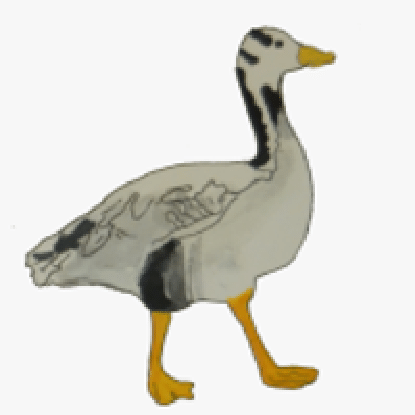
\includegraphics[width=3cm]{duck.png}
\tikz[remember picture,overlay]{\node[ellipse callout, draw, thick, fill=white, overlay, callout absolute pointer={($(-0.4,2.5)$)}] at ($(3.5,3.5)$) {\Large{I am a duck. Quack.}};}